\section{Why high switching frequency?}
\title[Why high switching frequency?]{Why high switching frequency?}

\begin{frame}[plain]
	\titlepage
\end{frame}

%%%%%%%%%%%%%%%%%%%%%%%%%%%%%%%%%%%%%%%%%%%%%%%%%%%%%%%%%%%%%
%% Course overview %%
%%%%%%%%%%%%%%%%%%%%%%%%%%%%%%%%%%%%%%%%%%%%%%%%%%%%%%%%%%%%%
\subsection{Course overview}

\begin{frame}
	\frametitle{Course overview}
	The course is organised in seven modules.
	\begin{itemize}
		\item Module A: Foundations -- why high frequency and what changes (L1--L2).
		\item Module B: The HF commutation cell in practice -- layout, gate drive, measurement (L3--L5).
		\item Module C: High-frequency magnetics (L6--L7).
		\item Module D: Soft-switching and resonant topologies (L8--L10).
		\item Module E: Case studies and teardown (L11).
		\item Module F: Capacitive conversion, control and system design (L12--L14).
		\item Module G: Synthesis and exam preparation (L15).
	\end{itemize}
	\textbf{Pattern of class}: \\
	Lecture: Tuesday, 12--14 \\
	Tutorial: Wednesday, 08--10 (numericals and Jupyter notebooks) \\
	Design clinic and lab: Wednesday, 10--12 (milestone reviews, hardware track)
\end{frame}

%%%%%%%%%%%%%%%%%%%%%%%%%%%%%%%%%%%%%%%%%%%%%%%%%%%%%%%%%%%%%
%% Frequency ladder %%
%%%%%%%%%%%%%%%%%%%%%%%%%%%%%%%%%%%%%%%%%%%%%%%%%%%%%%%%%%%%%
\begin{frame}
	\frametitle{The frequency ladder}
	\begin{figure}
		\centering
		\begin{tikzpicture}[
				rung/.style={draw, rounded corners=2pt, minimum width=1.9cm, minimum height=0.75cm, font=\small\bfseries},
				limit/.style={draw, rounded corners=2pt, text width=6.6cm, align=left, font=\footnotesize, minimum height=0.75cm, inner sep=3pt},
			]
			% rails of the ladder
			\draw[line width=1.5pt, gray] (-1.25,-0.5) -- (-1.25,4.4);
			\draw[line width=1.5pt, gray] (1.25,-0.5) -- (1.25,4.4);
			% rungs
			\foreach \y/\f in {0/{100\,kHz}, 1.3/{1\,MHz}, 2.6/{10\,MHz}, 3.9/{100\,MHz}} {
					\node[rung, fill=white] at (0,\y) {\f};
				}
			% what limits the design at each rung
			\node[limit, anchor=west] at (2.0,0) {\textbf{Switching loss:} $V$--$I$ overlap, $Q_\mathrm{oss}V$, $Q_\mathrm{rr}V$, gate charge};
			\node[limit, anchor=west] at (2.0,1.3) {\textbf{Parasitics and timing:} loop inductance, ringing, dead time, delays};
			\node[limit, anchor=west] at (2.0,2.6) {\textbf{Magnetics and devices:} core loss limits $\hat{B}$, skin and proximity effect, $C_\mathrm{oss}$ loss};
			\node[limit, anchor=west] at (2.0,3.9) {\textbf{Packaging, integration, control:} interconnects, sensing, latency};
			% lectures
			\node[font=\footnotesize, anchor=west] at (9.0,0) {L2, L8};
			\node[font=\footnotesize, anchor=west] at (9.0,1.3) {L3, L4, L5};
			\node[font=\footnotesize, anchor=west] at (9.0,2.6) {L6, L7, L9, L10};
			\node[font=\footnotesize, anchor=west] at (9.0,3.9) {L12, L13, L14};
			\node[font=\scriptsize\bfseries, anchor=west] at (9.0,4.55) {Lectures};
			\node[font=\scriptsize\bfseries, anchor=west] at (2.0,4.55) {Main limitation};
			\draw[-{Latex[length=3mm]}, thick] (-2.0,-0.4) -- node[sloped, above, font=\scriptsize] {$f_\mathrm{sw}\times 10$ per rung} (-2.0,4.4);
		\end{tikzpicture}
		\caption{The frequency ladder used throughout the course}
	\end{figure}
	Each lecture comes back to this ladder with one question: what breaks next when $f_\mathrm{sw}$ goes up by a factor of ten?
\end{frame}

%%%%%%%%%%%%%%%%%%%%%%%%%%%%%%%%%%%%%%%%%%%%%%%%%%%%%%%%%%%%%
%% Position of the course %%
%%%%%%%%%%%%%%%%%%%%%%%%%%%%%%%%%%%%%%%%%%%%%%%%%%%%%%%%%%%%%
\begin{frame}
	\frametitle{Relation to other courses}
	\begin{columns}[T]
		\begin{column}{0.46\textwidth}
			\begin{figure}
				\centering
				\begin{tikzpicture}[node distance=0.32cm,
						crs/.style={draw, rounded corners=2pt, align=center, font=\scriptsize, inner sep=3pt, text width=5.4cm, minimum height=1.0cm},
					]
					\node[crs] (pe) {\textbf{PE} (Power Electronics)\\ topologies, averaging, PWM, basic control};
					\node[crs, below=of pe] (pedc) {\textbf{PEDC} (Devices and Components)\\ Si/SiC/GaN devices, switching transients, magnetics and capacitor basics};
					\node[crs, below=of pedc, very thick] (hs) {\textbf{HSFPC} (this course)\\ what changes at MHz: soft switching, resonant/VHF and SC converters, HF magnetics, layout, gate drive, measurement, EMI, control};
					\draw[-{Latex[length=2mm]}, thick] (pe) -- (pedc);
					\draw[-{Latex[length=2mm]}, thick] (pedc) -- (hs);
				\end{tikzpicture}
				\caption{Course sequence}
			\end{figure}
		\end{column}
		\begin{column}{0.52\textwidth}
			\begin{itemize}
				\item The course builds on PE and PEDC.
				\item Device physics and basic magnetics are not repeated. Short recaps refer to the PEDC slides.
				\item If you did not attend PEDC, use the \textbf{bridge pack} in weeks 1--2: PEDC L05--L08 and PE L02--L03.
				\item ss
				\item The self-check at the end of this section tells you where to start.
			\end{itemize}
		\end{column}
	\end{columns}
\end{frame}

%%%%%%%%%%%%%%%%%%%%%%%%%%%%%%%%%%%%%%%%%%%%%%%%%%%%%%%%%%%%%
%% Learning objectives %%
%%%%%%%%%%%%%%%%%%%%%%%%%%%%%%%%%%%%%%%%%%%%%%%%%%%%%%%%%%%%%
\begin{frame}
	\frametitle{Learning objectives}
	After this course you can
	\begin{enumerate}
		\item quantify how passives, losses, parasitics, magnetics, EMI and control scale with the switching frequency for a given voltage, current and power, and justify a switching frequency,
		\item analyse soft-switched PWM, resonant, VHF and switched-capacitor converters with suitable models,
		\item design the HF commutation cell (devices, gate drive, layout) and HF magnetic and capacitive components,
		\item build and critically assess a complete loss budget and choose mitigations,
		\item use Python, SPICE, KiCad and sound measurement practice to design and verify HF converters,
		\item defend your design decisions orally, including what-if trade-offs.
	\end{enumerate}
\end{frame}

%%%%%%%%%%%%%%%%%%%%%%%%%%%%%%%%%%%%%%%%%%%%%%%%%%%%%%%%%%%%%
%% Design project and exam %%
%%%%%%%%%%%%%%%%%%%%%%%%%%%%%%%%%%%%%%%%%%%%%%%%%%%%%%%%%%%%%
\begin{frame}
	\frametitle{Design project and exam}
	\begin{columns}[T]
		\begin{column}{0.5\textwidth}
			\textbf{Design project} (teams of two, from week 4)
			\begin{itemize}
				\item Six briefs, all $\leq$ 60\,V DC, each team with its own parameter variant.
				\item Deliverable: design package with loss budget, component design, simulation with parasitics, KiCad layout and test plan.
				\item Optional hardware track on low-voltage GaN half-bridge boards.
			\end{itemize}
			\textbf{Voluntary milestones with feedback}\\
			{\footnotesize
				\begin{tabular}{lll}
					M0 & 11.11. & specification, topology, loss budget \\
					M1 & 25.11. & devices and magnetics pre-design      \\
					M2 & 16.12. & preliminary design review             \\
					M3 & 20.01. & layout and critical design review     \\
					M4 & 03.02. & final design package                  \\
				\end{tabular}}
		\end{column}
		\begin{column}{0.47\textwidth}
			\textbf{Oral exam on your own design} ($\approx$ 40\,min)
			\begin{itemize}
				\item Part A (10\,min): you present your design.
				\item Part B (20\,min): what-if questions with short calculations.
				\item Part C (10\,min): questions on L1--L14.
			\end{itemize}
			Measured results are not required for a top grade, a sound validation plan is.\\[0.5em]
			{\footnotesize The exam form is formally announced by 10.11.2026.}
		\end{column}
	\end{columns}
\end{frame}

%%%%%%%%%%%%%%%%%%%%%%%%%%%%%%%%%%%%%%%%%%%%%%%%%%%%%%%%%%%%%
%% Design briefs %%
%%%%%%%%%%%%%%%%%%%%%%%%%%%%%%%%%%%%%%%%%%%%%%%%%%%%%%%%%%%%%
\begin{frame}
	\frametitle{Design project briefs}
	\begin{table}
		\centering
		\footnotesize
		\begin{tabular}{|l|>{\raggedright\arraybackslash}p{3.4cm}|>{\raggedright\arraybackslash}p{4.3cm}|>{\raggedright\arraybackslash}p{5.2cm}|}
			\hline
			   & \textbf{Brief}                      & \textbf{Base specification}                           & \textbf{Main learning focus}                         \\
			\hline
			B1 & ZVS GaN buck (TCM/QSW)              & 48\,V $\rightarrow$ 12\,V, 100\,W, 1--3\,MHz             & ZVS, variable $f_\mathrm{sw}$, HF inductor, layout   \\
			\hline
			B2 & LLC DC transformer (DCX)            & 48\,V $\rightarrow$ 12\,V, 250\,W, $\approx$ 1\,MHz      & resonant tank, planar transformer, SR timing         \\
			\hline
			B3 & Bidirectional DAB                   & 48\,V $\leftrightarrow$ 12\,V, 200\,W, 0.5--1\,MHz      & ZVS range, leakage design, phase-shift control       \\
			\hline
			B4 & 6.78\,MHz wireless-power transmitter & 24\,V in, 15\,W into a given coil and load range        & class E or ZVS class D, coil Q, matching             \\
			\hline
			B5 & VHF dc--dc converter                & 12--24\,V $\rightarrow$ 5\,V, 5--10\,W, 13.56\,MHz       & class E/$\Phi_2$, resonant rectifier, air-core inductors \\
			\hline
			B6 & Resonant/hybrid SC converter        & 48\,V $\rightarrow$ 12\,V, 150\,W, $\leq$ 1\,MHz         & charge vectors, capacitor derating, soft charging    \\
			\hline
		\end{tabular}
		\caption{Design briefs (details in the project folder of the repository)}
	\end{table}
\end{frame}

%%%%%%%%%%%%%%%%%%%%%%%%%%%%%%%%%%%%%%%%%%%%%%%%%%%%%%%%%%%%%
%% Self-check %%
%%%%%%%%%%%%%%%%%%%%%%%%%%%%%%%%%%%%%%%%%%%%%%%%%%%%%%%%%%%%%
% The frame has two pages: questions only (page 1) and questions with answers (page 2).
\begin{frame}<handout:1-2>
	\frametitle{Self-check}
	\begin{varblock}[\textwidth]{Five questions from PE and PEDC}
		\small
		\renewcommand{\arraystretch}{1.15}
		\begin{tabular}{p{0.3cm}p{8.6cm}p{4.9cm}}
			1 & A buck converter in CCM converts 24\,V to 5\,V. Duty cycle $D$?
			  & \onslide<2-|handout:2>{$D=V_\mathrm{o}/V_\mathrm{in}\approx 0.21$} \\
			2 & Same buck, $L=10\,\mu$H, $f_\mathrm{sw}=500$\,kHz. Peak-to-peak inductor ripple?
			  & \onslide<2-|handout:2>{$\Delta I_L=\dfrac{V_\mathrm{o}(1-D)}{L f_\mathrm{sw}}\approx 0.79$\,A} \\
			3 & Hard switching at 48\,V, 10\,A, $t_\mathrm{r}+t_\mathrm{f}=20$\,ns, 500\,kHz. Overlap loss?
			  & \onslide<2-|handout:2>{$\frac12 VI(t_\mathrm{r}+t_\mathrm{f})f_\mathrm{sw}=2.4$\,W} \\
			4 & You double the turns of a gapped inductor (same core, same gap). Inductance?
			  & \onslide<2-|handout:2>{$L=N^2/\mathcal{R}$: four times} \\
			5 & A $\pm V$ square wave: amplitude of the 3rd harmonic relative to the fundamental?
			  & \onslide<2-|handout:2>{$1/3$, since $\hat{v}_n=\frac{4V}{\pi n}$ (odd $n$)} \\
		\end{tabular}
	\end{varblock}
	\onslide<2-|handout:2>{\small Two or more wrong? Work through the bridge pack in weeks 1--2: PE L02--L03 (Q1, Q2), PEDC L05--L06 (Q3), PEDC L07 (Q4), PE L04 (Q5).}
\end{frame}

%%%%%%%%%%%%%%%%%%%%%%%%%%%%%%%%%%%%%%%%%%%%%%%%%%%%%%%%%%%%%
%% Motivation %%
%%%%%%%%%%%%%%%%%%%%%%%%%%%%%%%%%%%%%%%%%%%%%%%%%%%%%%%%%%%%%
\subsection{Motivation and examples}

\begin{frame}
	\frametitle{Why increase the switching frequency?}
	\begin{columns}[T]
		\begin{column}{0.52\textwidth}
			\small
			\textbf{What we want}
			\begin{itemize}
				\item smaller and lighter converters
				\item more bandwidth: faster regulation and transients
				\item integration into packages and chips
				\item new applications: wireless power, RF power
				\item eventually, lower cost
			\end{itemize}
			\textbf{Why frequency helps}
			\begin{itemize}
				\item energy stored per cycle $\propto 1/f_\mathrm{sw}$, hence $L, C \propto 1/f_\mathrm{sw}$
				\item passive components dominate size, weight and loss, magnetics are the hardest part
			\end{itemize}
		\end{column}
		\begin{column}{0.45\textwidth}
			\begin{block}{Half a century of progress}
				Power density of converters has roughly doubled every 10 years since 1970. The devices behind it raised $f_\mathrm{sw}$ by about a factor of 10 per decade.\\[0.4em]
				Rule of thumb: doubling the power density typically needs about 10 times higher $f_\mathrm{sw}$.
			\end{block}
		\end{column}
	\end{columns}
	\blfootnote{Sources: Perreault, APEC 2024 plenary; Kolar et al., IEEJ Trans. Ind. Appl., 2008.}
\end{frame}

%%%%%%%%%%%%%%%%%%%%%%%%%%%%%%%%%%%%%%%%%%%%%%%%%%%%%%%%%%%%%
%% Quiz: guess the switching frequency %%
%%%%%%%%%%%%%%%%%%%%%%%%%%%%%%%%%%%%%%%%%%%%%%%%%%%%%%%%%%%%%
% Two pages: guesses (page 1) and actual values (page 2).
\begin{frame}<handout:1-2>
	\frametitle{Switching frequency quiz}
	For each product, guess $f_\mathrm{sw}$ (one decade is fine) and name the constraint that sets the ceiling. Discuss with your neighbour (3 minutes).
	\begin{table}
		\centering
		\small
		\begin{tabular}{|r|l|l|l|}
			\hline
			  & \textbf{Product}                                          & \textbf{Rating}               & \onslide<2-|handout:2>{\textbf{Actual} $f_\mathrm{sw}$} \\
			\hline
			1 & On-die voltage regulator in a CPU                         & whole CPU, laptop to server   & \onslide<2-|handout:2>{140\,MHz}   \\
			2 & 48\,V-to-1\,V CPU regulator module                        & 240\,A                        & \onslide<2-|handout:2>{1.5\,MHz}   \\
			3 & Data-centre DC transformer 380\,V $\rightarrow$ 12\,V      & 1\,kW                         & \onslide<2-|handout:2>{1\,MHz}     \\
			4 & Mains-powered LED driver (120\,V AC)                      & 30\,W                         & \onslide<2-|handout:2>{5--10\,MHz} \\
			5 & Inductive wireless power link                             & 1\,kW                         & \onslide<2-|handout:2>{6.78\,MHz}  \\
			6 & SiC CLLC dc--dc stage (IAS research model)                & 11\,kW                        & \onslide<2-|handout:2>{125\,kHz}   \\
			\hline
		\end{tabular}
	\end{table}
	\onslide<2-|handout:2>{$f_\mathrm{sw}$ spans three decades and neither power nor voltage alone predicts it. The ceilings differ: interconnect and conduction at high current (1, 2), capacitive switching energy at high voltage (3, 6), magnetics and EMI everywhere.}
	\blfootnote{(1) Burton et al., APEC 2014 (Intel FIVR); (2) Elasser et al., APEC 2023; (3) Ranjram and Perreault, TPEL 2022; (4) Lim, Otten and Perreault, TPEL 2016; (5) Gu et al., TPEL 2021; (6) IAS LTspice model.}
\end{frame}

%%%%%%%%%%%%%%%%%%%%%%%%%%%%%%%%%%%%%%%%%%%%%%%%%%%%%%%%%%%%%
%% MHz converters today %%
%%%%%%%%%%%%%%%%%%%%%%%%%%%%%%%%%%%%%%%%%%%%%%%%%%%%%%%%%%%%%
\begin{frame}
	\frametitle{MHz converters today}
	\begin{table}
		\centering
		\scriptsize
		\setlength{\tabcolsep}{3pt}
		\begin{tabular}{|>{\raggedright\arraybackslash}p{3.75cm}|l|l|>{\raggedright\arraybackslash}p{4.3cm}|l|}
			\hline
			\textbf{Application}                        & \textbf{Power} & \textbf{$f_\mathrm{sw}$} & \textbf{Key figure}                     & \textbf{Source}                \\
			\hline
			On-die CPU buck regulators                  & whole CPU      & 140\,MHz                 & Intel FIVR, air-core inductors          & Burton 2014                    \\
			48\,V $\rightarrow$ 1\,V CPU regulator      & 240\,W         & 1.5\,MHz                 & 1390\,W/in$^3$, 8.4\,mm high            & Elasser 2023                   \\
			380\,V $\rightarrow$ 12\,V DC transformer   & 1\,kW          & 1\,MHz                   & 97.1\,\% at full load                   & Ranjram 2022                   \\
			120\,V AC LED driver                        & 30\,W          & 5--10\,MHz               & 50\,W/in$^3$, meets FCC Class B         & Lim 2016$^{*}$                 \\
			Universal-input PFC supply                  & 250\,W         & 1--4\,MHz                & 95.3\,\%, EMI filter 8\,\% of volume    & Santiago-Gonz\'alez 2023$^{*}$ \\
			Inductive wireless power                    & 1\,kW          & 6.78\,MHz                & 95\,\% dc--dc                           & Gu 2021$^{*}$                  \\
			Industrial RF power inverter                & 5\,kW          & 13.56\,MHz               & ISM band                                & Zhang 2022$^{*}$               \\
			\hline
			\multicolumn{5}{|l|}{\textit{For comparison}}                                                                                                     \\
			EV battery charger                          & 18\,kW         & 500\,kHz                 & 98.8\,\% efficiency                     & Cao 2022                       \\
			IAS SiC CLLC dc--dc stage                   & 11\,kW         & 125\,kHz                 & our running example (L9, L11)           & IAS model                      \\
			\hline
		\end{tabular}
		\caption{Published designs in the MHz range ($^{*}$as summarised by Perreault, APEC 2024; full references at the end of the lecture)}
	\end{table}
	Today, kW converters run at low MHz and tens of watts at tens of MHz. The open opportunity is the kW scale at 10\,MHz and beyond.
\end{frame}

%%%%%%%%%%%%%%%%%%%%%%%%%%%%%%%%%%%%%%%%%%%%%%%%%%%%%%%%%%%%%
%% Power-frequency map %%
%%%%%%%%%%%%%%%%%%%%%%%%%%%%%%%%%%%%%%%%%%%%%%%%%%%%%%%%%%%%%
\begin{frame}
	\frametitle{Power--frequency map}
	\begin{columns}[T]
		\begin{column}{0.62\textwidth}
			\begin{figure}
				\centering
				\begin{tikzpicture}
					\begin{loglogaxis}[
							width=0.97\linewidth, height=6.0cm,
							xmin=1, xmax=1e5, ymin=1e4, ymax=1e9,
							xlabel={Output power (W)}, ylabel={Switching frequency (Hz)},
							grid=major, grid style={gray!20},
							tick label style={font=\scriptsize}, label style={font=\footnotesize},
							legend style={at={(0.02,0.02)}, anchor=south west, font=\tiny, row sep=-1pt},
							legend cell align=left,
						]
						% band of present designs and the opportunity
						\fill[gray!12] (axis cs:30,3e5) rectangle (axis cs:2e4,4e6);
						\node[font=\tiny, anchor=north east] at (axis cs:1.9e4,3.9e6) {kW at low MHz};
						\draw[-{Latex[length=2.5mm]}, thick] (axis cs:1.2e4,5e6) -- (axis cs:1.2e4,5e7)
						node[font=\tiny, anchor=east] {kW at 10+\,MHz?};
						% published designs
						\addplot[only marks, mark=square*, mark size=1.8pt] coordinates {(240,1.5e6) (1000,1e6)};
						\addlegendentry{data centre, CPU}
						\addplot[line width=2pt, forget plot] coordinates {(10,1.4e8) (150,1.4e8)};
						\addplot[only marks, mark=*, mark size=1.8pt] coordinates {(30,7.07e6) (250,2e6)};
						\addlegendentry{mains-powered supplies}
						\addplot[line width=1.2pt, forget plot] coordinates {(30,5e6) (30,1e7)};
						\addplot[line width=1.2pt, forget plot] coordinates {(250,1e6) (250,4e6)};
						\addplot[only marks, mark=triangle, mark size=2.6pt] coordinates {(1000,6.78e6) (3000,3.39e6) (3700,1.356e7)};
						\addlegendentry{wireless power}
						\addplot[only marks, mark=diamond, mark size=2.6pt] coordinates {(1000,1.356e7) (1500,1.356e7) (5000,1.356e7)};
						\addlegendentry{RF power}
						\addplot[only marks, mark=o, mark size=2.2pt] coordinates {(18000,5e5) (11000,1.25e5) (5000,3e5) (10000,8.2e5)};
						\addlegendentry{kW dc--dc and PFC}
						\fill[gray!30] (axis cs:3300,2e4) rectangle (axis cs:22000,1e5);
						% labels
						\node[font=\tiny, anchor=south] at (axis cs:39,1.6e8) {on-die regulators};
						\node[font=\tiny, anchor=east] at (axis cs:200,1.4e6) {CPU module};
						\node[font=\tiny, anchor=north] at (axis cs:1000,0.9e6) {DCX};
						\node[font=\tiny, anchor=east] at (axis cs:27,7e6) {LED};
						\node[font=\tiny, anchor=south] at (axis cs:250,4.2e6) {PFC};
						\node[font=\tiny, anchor=west] at (axis cs:12500,1.25e5) {IAS CLLC};
						\node[font=\tiny] at (axis cs:8500,4.4e4) {Si OBC};
					\end{loglogaxis}
				\end{tikzpicture}
				\caption{Published designs (previous slide; Perreault 2024; Kolar 2008; Zhang 2025) on the power--frequency plane}
			\end{figure}
		\end{column}
		\begin{column}{0.36\textwidth}
			\small
			\begin{itemize}
				\item Each point is a published design, not a limit.
				\item Lower power allows higher $f_\mathrm{sw}$: smaller devices, smaller loops, less energy per switching edge.
				\item Classical kW designs have their volume optimum at a few hundred kHz, because cooling grows with $f_\mathrm{sw}$ while passives shrink.
				\item Moving up the map needs new topologies, magnetics and devices.
			\end{itemize}
		\end{column}
	\end{columns}
\end{frame}

%%%%%%%%%%%%%%%%%%%%%%%%%%%%%%%%%%%%%%%%%%%%%%%%%%%%%%%%%%%%%
%% Voltage and current limits %%
%%%%%%%%%%%%%%%%%%%%%%%%%%%%%%%%%%%%%%%%%%%%%%%%%%%%%%%%%%%%%
\begin{frame}
	\frametitle{Voltage and current limits}
	\begin{columns}[T]
		\begin{column}{0.48\textwidth}
			\begin{block}{Low voltage, high current}
				e.g.\ 48\,V $\rightarrow$ 1\,V at 240\,A
				\begin{itemize}
					\item conduction and interconnect: $P=I^2R_\mathrm{ac}(f_\mathrm{sw})$
					\item loop inductance: $v_L=L_\mathrm{loop}\,\mathrm{d}i/\mathrm{d}t$
					\item large dies, hence large $C_\mathrm{oss}$ and $Q_\mathrm{G}$
					\item winding and termination loss in transformers
				\end{itemize}
				Typical answers: many phases, matrix and fractional-turn transformers, vertical power delivery.
			\end{block}
		\end{column}
		\begin{column}{0.48\textwidth}
			\begin{block}{High voltage}
				e.g.\ 400\,V bus at 1\,kW
				\begin{itemize}
					\item capacitive switching loss: $P=Q_\mathrm{oss}V f_\mathrm{sw}$, $\propto V^2$ for a linear $C_\mathrm{oss}$
					\item $\mathrm{d}v/\mathrm{d}t$ drives common-mode current $i=C\,\mathrm{d}v/\mathrm{d}t$
					\item creepage and clearance distances enlarge the loops
					\item $C_\mathrm{oss}$ hysteresis, dynamic $R_\mathrm{DS(on)}$ (GaN)
				\end{itemize}
				Typical answers: zero-voltage switching, resonant converters, careful insulation design.
			\end{block}
		\end{column}
	\end{columns}
	\vspace{0.1cm}
	{\small Parasitic inductance grows with current (device area) and spacing grows with voltage. Both lower the ceiling at high power.}
\end{frame}

%%%%%%%%%%%%%%%%%%%%%%%%%%%%%%%%%%%%%%%%%%%%%%%%%%%%%%%%%%%%%
%% Your turn: hard switching at MHz %%
%%%%%%%%%%%%%%%%%%%%%%%%%%%%%%%%%%%%%%%%%%%%%%%%%%%%%%%%%%%%%
% Two pages: task (page 1) and task with solution (page 2).
\begin{frame}<handout:1-2>
	\frametitle{Hard switching at MHz}
	\begin{block}{Task (4 minutes)}
		A 650\,V GaN transistor has $Q_\mathrm{oss}=40$\,nC at 400\,V. In a half-bridge it turns on hard once per period: the opposite switch's $C_\mathrm{oss}$ is charged through its channel.
		\begin{enumerate}
			\item Capacitive switching loss at 100\,kHz and at 1\,MHz?
			\item Up to which $f_\mathrm{sw}$ does it stay below 1\,\% of a 1\,kW output?
			\item What would you change?
		\end{enumerate}
	\end{block}
	\onslide<2-|handout:2>{
		\begin{columns}[T]
			\begin{column}{0.52\textwidth}
				\begin{enumerate}
					\item $P=Q_\mathrm{oss}V_\mathrm{DC}f_\mathrm{sw}$: 1.6\,W at 100\,kHz, 16\,W at 1\,MHz.
					\item $f_\mathrm{sw}\leq\dfrac{10\,\mathrm{W}}{40\,\mathrm{nC}\cdot 400\,\mathrm{V}}=625$\,kHz.
					\item Let the load current charge $C_\mathrm{oss}$ before turn-on, i.e.\ zero-voltage switching (L8--L10).
				\end{enumerate}
			\end{column}
			\begin{column}{0.45\textwidth}
				\begin{block}{Note}
					\footnotesize The loss is $Q_\mathrm{oss}V_\mathrm{DC}$ for any shape of $C_\mathrm{oss}(v)$: the energy drawn from the bus ends up as heat in the switch that turns on. Using $\frac12 CV^2$ with a small-signal $C_\mathrm{oss}$ underestimates it.
				\end{block}
			\end{column}
		\end{columns}
	}
\end{frame}

%%%%%%%%%%%%%%%%%%%%%%%%%%%%%%%%%%%%%%%%%%%%%%%%%%%%%%%%%%%%%
%% Power density optimum %%
%%%%%%%%%%%%%%%%%%%%%%%%%%%%%%%%%%%%%%%%%%%%%%%%%%%%%%%%%%%%%
\begin{frame}
	\frametitle{Power density and optimum switching frequency}
	\begin{columns}[T]
		\begin{column}{0.48\textwidth}
			\begin{figure}
				\centering
				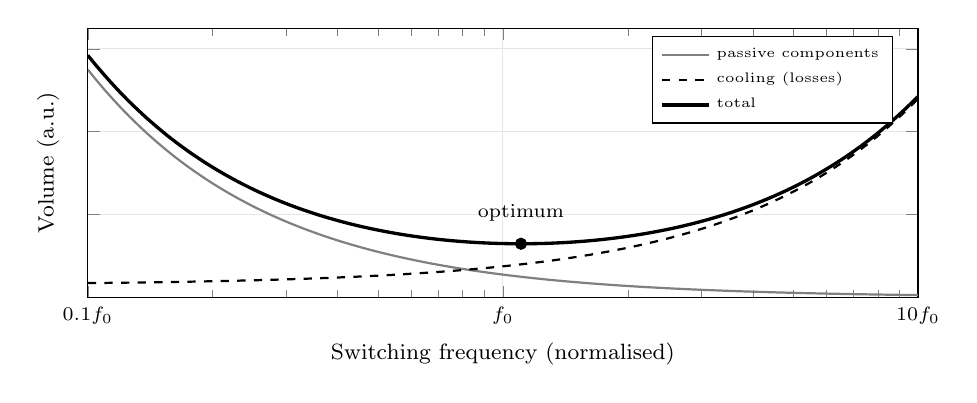
\begin{tikzpicture}
					\begin{semilogxaxis}[
							width=\linewidth, height=5.0cm,
							xmin=0.1, xmax=10, ymin=0, ymax=6.5,
							xlabel={Switching frequency (normalised)}, ylabel={Volume (a.u.)},
							xtick={0.1,1,10}, xticklabels={$0.1f_0$,$f_0$,$10f_0$}, yticklabels={},
							grid=major, grid style={gray!20},
							tick label style={font=\scriptsize}, label style={font=\footnotesize},
							legend style={font=\tiny}, legend pos=north east, legend cell align=left,
						]
						\addplot[gray, thick, domain=0.1:10, samples=100] {0.55/x};
						\addlegendentry{passive components}
						\addplot[black, thick, dashed, domain=0.1:10, samples=100] {0.3+0.45*x};
						\addlegendentry{cooling (losses)}
						\addplot[black, very thick, domain=0.1:10, samples=200] {0.55/x+0.3+0.45*x};
						\addlegendentry{total}
						\addplot[only marks, mark=*, mark size=2pt, forget plot] coordinates {(1.1055,1.295)};
						\node[font=\scriptsize, anchor=south] at (axis cs:1.1055,1.6) {optimum};
					\end{semilogxaxis}
				\end{tikzpicture}
				\caption{Qualitative trade-off: passive volume falls with $1/f_\mathrm{sw}$, the heat sink grows with the switching losses}
			\end{figure}
		\end{column}
		\begin{column}{0.5\textwidth}
			\small
			Volume-optimal $f_\mathrm{sw}$ of classical designs:
			\begin{itemize}
				\item 5\,kW isolated dc--dc converter: 28\,kW/dm$^3$ at 300\,kHz
				\item 10\,kW three-phase PFC rectifier: 44\,kW/dm$^3$ at 820\,kHz
			\end{itemize}
			Efficiency $\eta$ and power density $\rho$ conflict. Each design on the $\eta$--$\rho$ Pareto front is optimal for some weighting, and $f_\mathrm{sw}$ is one of the design variables.\\[0.3em]
			\textbf{Little Box Challenge} (Google/IEEE, 2014--16): 2\,kVA PV inverter, $\eta_\mathrm{CEC}>95\,\%$, case below 60\,$^\circ$C, target above 50\,W/in$^3$ ($\approx$ 3\,kW/dm$^3$). An ETH design study later reached 14.7\,kW/dm$^3$ at 98.1\,\% efficiency.
		\end{column}
	\end{columns}
	\blfootnote{Sources: Kolar et al., IEEJ Trans. Ind. Appl., 2008; Neumayr et al., CPSS Trans. Power Electron. Appl., vol. 5, no. 2, 2020.}
\end{frame}

%%%%%%%%%%%%%%%%%%%%%%%%%%%%%%%%%%%%%%%%%%%%%%%%%%%%%%%%%%%%%
%% What gets smaller with frequency %%
%%%%%%%%%%%%%%%%%%%%%%%%%%%%%%%%%%%%%%%%%%%%%%%%%%%%%%%%%%%%%
\subsection{What gets smaller with frequency}

\begin{frame}
	\frametitle{Energy per switching cycle}
	\begin{columns}[T]
		\begin{column}{0.5\textwidth}
			\begin{figure}
				\centering
				\begin{circuitikz}[scale=0.74, transform shape]
					\draw (0,0) to[V, l=$V_\mathrm{in}$] (0,2.6)
					to[short] (0.4,2.6) to[nos, l=$S_1$] (2.2,2.6)
					to[short, -*] (2.6,2.6) coordinate (sw)
					to[L, l=$L$, i>^=$i_L$] (4.8,2.6)
					to[short, -*] (5.2,2.6) coordinate (out)
					to[short] (6.6,2.6) to[R, l=$R$] (6.6,0) -- (0,0);
					\draw (sw) to[nos, l_=$S_2$] (2.6,0) node[circ] {};
					\draw (out) to[C, l_=$C$] (5.2,0) node[circ] {};
					\draw (7.4,2.6) to[open, v^=$V_\mathrm{o}$] (7.4,0);
				\end{circuitikz}
				\caption{Buck converter in continuous conduction mode (CCM)}
			\end{figure}
			Energy processed per cycle: $W=P/f_\mathrm{sw}$, e.g.\ 100\,W at 100\,kHz $\rightarrow$ 1\,mJ, at 10\,MHz $\rightarrow$ 10\,$\mu$J.
		\end{column}
		\begin{column}{0.47\textwidth}
			For a given current ripple $\Delta I_L$ and voltage ripple $\Delta V_\mathrm{o}$ (CCM):
			\begin{align*}
				L & =\frac{V_\mathrm{o}(1-D)}{f_\mathrm{sw}\,\Delta I_L}\propto\frac{1}{f_\mathrm{sw}} \\
				C & =\frac{\Delta I_L}{8 f_\mathrm{sw}\,\Delta V_\mathrm{o}}\propto\frac{1}{f_\mathrm{sw}}
			\end{align*}
			The peak inductor energy $\frac12 L\hat{i}_L^2$ falls with $1/f_\mathrm{sw}$ as well, since $\hat{i}_L=I_\mathrm{o}+\Delta I_L/2$ is fixed.
		\end{column}
	\end{columns}
	\begin{block}{Key message}
		Higher $f_\mathrm{sw}$ reduces the required inductance and capacitance. It does not automatically reduce the size of the component.
	\end{block}
\end{frame}

%%%%%%%%%%%%%%%%%%%%%%%%%%%%%%%%%%%%%%%%%%%%%%%%%%%%%%%%%%%%%
%% Your turn: buck inductor at 100 kHz and 2 MHz %%
%%%%%%%%%%%%%%%%%%%%%%%%%%%%%%%%%%%%%%%%%%%%%%%%%%%%%%%%%%%%%
\begin{frame}<handout:1-2>
	\frametitle{Buck inductor sizing}
	\begin{block}{Task (4 minutes)}
		Buck converter 48\,V $\rightarrow$ 12\,V, 10\,A, inductor ripple $\Delta I_L=3$\,A (30\,\%), output ripple $\Delta V_\mathrm{o}=120$\,mV (1\,\%).
		\begin{enumerate}
			\item Calculate $L$ and $C$ at 100\,kHz and at 2\,MHz.
			\item Is the 2\,MHz inductor 20 times smaller?
		\end{enumerate}
	\end{block}
	\onslide<2-|handout:2>{
		\begin{enumerate}
			\item $D=0.25$: $L=30\,\mu$H $\rightarrow$ 1.5\,$\mu$H and $C=31.3\,\mu$F $\rightarrow$ 1.56\,$\mu$F.
			\item No, far from it:
			      \begin{itemize}
				      \item the winding still carries 10\,A DC, so the conductor cross-section does not shrink with $f_\mathrm{sw}$;
				      \item same core with $\sqrt{20}$ fewer turns: $\Delta B$ falls by $\sqrt{20}$, but the core loss density $\propto f^{\alpha}\Delta B^{\beta}$ rises by $20^{1.5}\cdot 20^{-1.3}\approx 1.8$ (ferrite, $\alpha\approx1.5$, $\beta\approx2.6$);
				      \item the skin depth falls from 209\,$\mu$m to 47\,$\mu$m, so the AC resistance of the winding rises.
			      \end{itemize}
			      The magnetics frames later in this lecture explain why.
		\end{enumerate}
	}
\end{frame}

%%%%%%%%%%%%%%%%%%%%%%%%%%%%%%%%%%%%%%%%%%%%%%%%%%%%%%%%%%%%%
%% EMI filter and control bandwidth %%
%%%%%%%%%%%%%%%%%%%%%%%%%%%%%%%%%%%%%%%%%%%%%%%%%%%%%%%%%%%%%
\begin{frame}
	\frametitle{EMI filter and control bandwidth}
	\begin{columns}[T]
		\begin{column}{0.5\textwidth}
			\begin{figure}
				\centering
				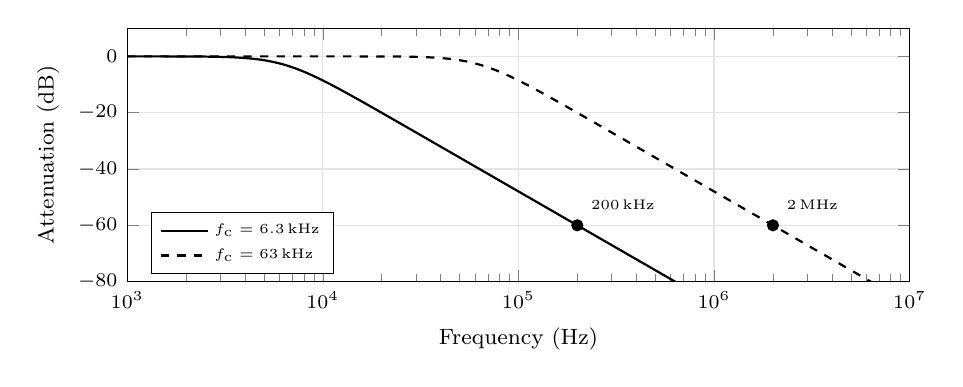
\begin{tikzpicture}
					\begin{semilogxaxis}[
							width=0.95\linewidth, height=4.8cm,
							xmin=1e3, xmax=1e7, ymin=-80, ymax=10,
							xlabel={Frequency (Hz)}, ylabel={Attenuation (dB)},
							grid=major, grid style={gray!20},
							tick label style={font=\scriptsize}, label style={font=\footnotesize},
							legend style={font=\tiny}, legend pos=south west, legend cell align=left,
						]
						\addplot[black, thick, domain=3:7, samples=200] ({10^x}, {-10*log10((1-(10^x/6324.6)^2)^2+(1.4*10^x/6324.6)^2)});
						\addlegendentry{$f_\mathrm{c}=6.3$\,kHz}
						\addplot[black, thick, dashed, domain=3:7, samples=200] ({10^x}, {-10*log10((1-(10^x/63246)^2)^2+(1.4*10^x/63246)^2)});
						\addlegendentry{$f_\mathrm{c}=63$\,kHz}
						\addplot[only marks, mark=*, mark size=2pt, forget plot] coordinates {(2e5,-60) (2e6,-60)};
						\node[font=\tiny, anchor=south west] at (axis cs:2.1e5,-58) {200\,kHz};
						\node[font=\tiny, anchor=south west] at (axis cs:2.1e6,-58) {2\,MHz};
					\end{semilogxaxis}
				\end{tikzpicture}
				\caption{Second-order LC filter ($\zeta=0.7$) providing 60\,dB at $f_\mathrm{sw}$}
			\end{figure}
		\end{column}
		\begin{column}{0.47\textwidth}
			\small
			\textbf{EMI filter:} the filter must attenuate the lowest switching harmonic in the regulated band (150\,kHz--30\,MHz for conducted emissions). With $-40$\,dB/dec, a filter giving $A$ (dB) at $f_\mathrm{sw}$ has its corner at $f_\mathrm{c}=f_\mathrm{sw}/10^{A/40}$. Ten times $f_\mathrm{sw}$ allows ten times $f_\mathrm{c}$, i.e.\ 100 times smaller $LC$. Perreault: ``It's not a bug, it's a feature!''\\[0.4em]
			\textbf{Control:} the crossover frequency $f_\mathrm{co}$ is typically $f_\mathrm{sw}/10$ to $f_\mathrm{sw}/5$. Near crossover $Z_\mathrm{out}\approx 1/(2\pi f_\mathrm{co}C)$, so a 100\,A load step with 30\,mV deviation needs 10.6\,mF at $f_\mathrm{co}=50$\,kHz but only 1.06\,mF at 500\,kHz.
		\end{column}
	\end{columns}
	\blfootnote{Source: Perreault, APEC 2024 plenary.}
\end{frame}

%%%%%%%%%%%%%%%%%%%%%%%%%%%%%%%%%%%%%%%%%%%%%%%%%%%%%%%%%%%%%
%% What does not shrink %%
%%%%%%%%%%%%%%%%%%%%%%%%%%%%%%%%%%%%%%%%%%%%%%%%%%%%%%%%%%%%%
\subsection{What does not shrink so easily}

\begin{frame}
	\frametitle{Scaling laws of magnetics}
	\begin{columns}[T]
		\begin{column}{0.5\textwidth}
			\begin{figure}
				\centering
				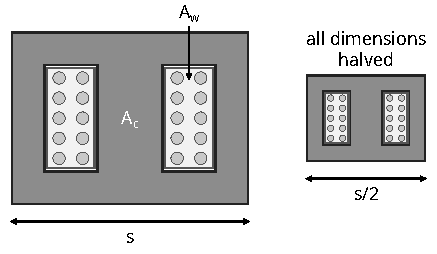
\includegraphics[width=\linewidth]{fig/lec01/core_scaling.pdf}
				\caption{An EE core scaled by $\alpha=1/2$ in every dimension ($A_\mathrm{c}$: core cross-section, $A_\mathrm{w}$: winding window)}
			\end{figure}
		\end{column}
		\begin{column}{0.47\textwidth}
			Power handling of a core with flux density $\hat{B}$ and current density $J$ (both set by losses):
			\begin{equation*}
				VA\propto f\,\hat{B}\,J\,A_\mathrm{c}A_\mathrm{w}
			\end{equation*}
			Scaling all dimensions by $\alpha$:
			\begin{itemize}
				\item $A_\mathrm{c}A_\mathrm{w}\propto\alpha^4$, volume $\propto\alpha^3$
				\item power density $\propto\alpha$: smaller is worse
				\item at constant loss density, loss/$VA\propto 1/\alpha$
			\end{itemize}
			Example: 100 transformers of 1\,W instead of one of 100\,W need $\alpha=100^{-1/4}\approx0.32$, i.e.\ $100\,\alpha^3\approx3.2$ times the volume and, at the same loss density, 3.2 times the loss.
		\end{column}
	\end{columns}
	\blfootnote{Source: C.\,R. Sullivan et al., ``On size and magnetics: Why small efficient power inductors are rare,'' 3D-PEIM 2016.}
\end{frame}

\begin{frame}
	\frametitle{Performance factor of magnetic materials}
	\begin{columns}[T]
		\begin{column}{0.5\textwidth}
			\begin{figure}
				\centering
				\begin{tikzpicture}
					\begin{semilogxaxis}[
							width=\linewidth, height=4.3cm,
							xmin=1.5, xmax=25, ymin=0, ymax=160,
							xtick={2,5,10,20}, xticklabels={2,5,10,20},
							xlabel={Frequency (MHz)}, ylabel={$\hat{B}f$ (mT$\cdot$MHz)},
							grid=major, grid style={gray!20},
							tick label style={font=\scriptsize}, label style={font=\footnotesize},
							legend style={font=\tiny, at={(0.5,-0.4)}, anchor=north, legend columns=2, /tikz/every even column/.append style={column sep=0.25cm}}, legend cell align=left,
							unbounded coords=jump,
						]
						\addplot[black, thick, mark=*, mark size=1.5pt] table[x=f_MHz, y=FR67] {fig/lec01/data/pf_hanson2016_Pv500.dat};
						\addlegendentry{67, $\mu_\mathrm{r}=40$}
						\addplot[black, thick, dashed, mark=square*, mark size=1.5pt] table[x=f_MHz, y=M3] {fig/lec01/data/pf_hanson2016_Pv500.dat};
						\addlegendentry{M3, $\mu_\mathrm{r}=20$}
						\addplot[gray, thick, mark=triangle*, mark size=1.8pt] table[x=f_MHz, y=F4F1] {fig/lec01/data/pf_hanson2016_Pv500.dat};
						\addlegendentry{4F1, $\mu_\mathrm{r}=80$}
						\addplot[gray, thick, dashed, mark=o, mark size=1.5pt] table[x=f_MHz, y=FR61] {fig/lec01/data/pf_hanson2016_Pv500.dat};
						\addlegendentry{61, $\mu_\mathrm{r}=125$}
					\end{semilogxaxis}
				\end{tikzpicture}
				\caption{Performance factor at $P_\mathrm{v}=500$\,mW/cm$^3$ from the Steinmetz fits of Hanson et al.\ (2016): Fair-Rite 67, 61; Nat.\ Magnetics M3; Ferroxcube 4F1}
			\end{figure}
		\end{column}
		\begin{column}{0.47\textwidth}
			\small
			At high frequency $\hat{B}$ is limited by core loss, not by saturation. With the Steinmetz fit $P_\mathrm{v}=k\hat{B}^{\beta}$ at each frequency:
			\begin{equation*}
				\hat{B}=\left(\frac{P_\mathrm{v}}{k}\right)^{1/\beta},\qquad PF=\hat{B}\,f
			\end{equation*}
			\begin{itemize}
				\item At fixed size and loss density, $VA\propto PF$.
				\item $PF$ rises with $f$ only up to a material-specific limit, here 10--15\,MHz.
				\item With available materials, $PF$ keeps improving up to about 30\,MHz (Perreault, 2024).
				\item With skin effect in a single-layer winding, $\hat{B}f^{3/4}$ is the fairer metric (L6).
			\end{itemize}
		\end{column}
	\end{columns}
\end{frame}

%%%%%%%%%%%%%%%%%%%%%%%%%%%%%%%%%%%%%%%%%%%%%%%%%%%%%%%%%%%%%
%% Device losses %%
%%%%%%%%%%%%%%%%%%%%%%%%%%%%%%%%%%%%%%%%%%%%%%%%%%%%%%%%%%%%%
\begin{frame}
	\frametitle{Power semiconductor devices}
	\begin{table}
		\centering
		\small
		\begin{tabular}{|l|l|>{\raggedright\arraybackslash}p{6.2cm}|}
			\hline
			\textbf{Mechanism}                    & \textbf{Energy per period}                  & \textbf{Remark}                                                     \\
			\hline
			$V$--$I$ overlap (hard switching)     & $\frac12 VI(t_\mathrm{r}+t_\mathrm{f})$      & set by drive strength, $\mathrm{d}i/\mathrm{d}t$, $\mathrm{d}v/\mathrm{d}t$ \\
			$C_\mathrm{oss}$ charging (hard turn-on) & $Q_\mathrm{oss}V_\mathrm{DC}$            & present even with an infinitely fast switch                         \\
			Reverse recovery                      & $\approx Q_\mathrm{rr}V_\mathrm{DC}$          & Si body diodes; none for GaN, small for SiC                         \\
			Gate drive (per switch)               & $Q_\mathrm{G}V_\mathrm{dr}$                  & dissipated in the driver and gate resistors                         \\
			Dead-time conduction                  & $2V_\mathrm{SD}I\,t_\mathrm{d}$              & GaN conducts in reverse at a few volts                              \\
			$C_\mathrm{oss}$ hysteresis           & $E_\mathrm{hyst}$                            & remains with soft switching, may exceed conduction loss at MHz      \\
			\hline
		\end{tabular}
		\caption{Switching-related loss mechanisms, all multiplied by $f_\mathrm{sw}$}
	\end{table}
	Conduction loss $I^2R_\mathrm{DS(on)}$ does not depend on $f_\mathrm{sw}$. Every term in the table does. L2 turns this table into a complete loss model.
	\blfootnote{$C_\mathrm{oss}$ hysteresis: Fedison et al., APEC 2014; Zulauf et al., TPEL 2018; Perreault, APEC 2024.}
\end{frame}

\begin{frame}
	\frametitle{Switching versus conduction loss}
	\begin{columns}[T]
		\begin{column}{0.55\textwidth}
			\begin{figure}
				\centering
				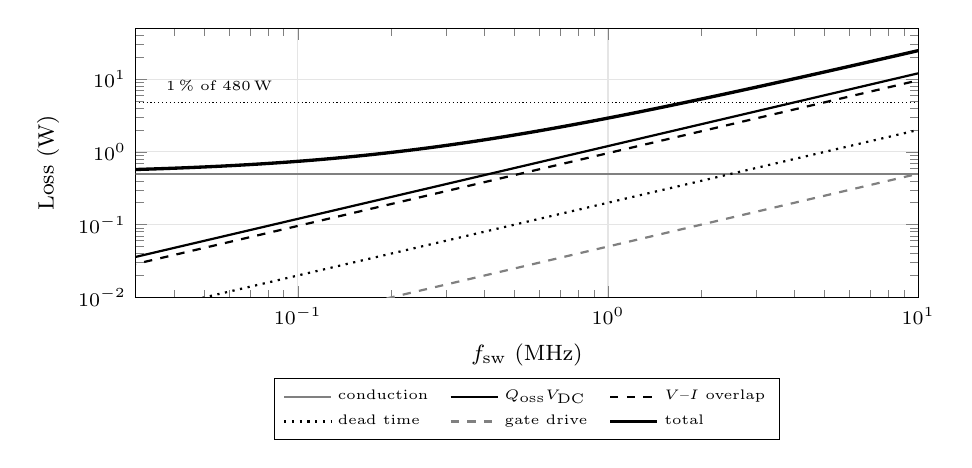
\begin{tikzpicture}
					\begin{loglogaxis}[
							width=0.95\linewidth, height=5.0cm,
							xmin=0.03, xmax=10, ymin=0.01, ymax=50,
							xlabel={$f_\mathrm{sw}$ (MHz)}, ylabel={Loss (W)},
							grid=major, grid style={gray!20},
							tick label style={font=\scriptsize}, label style={font=\footnotesize},
							legend style={font=\tiny, at={(0.5,-0.3)}, anchor=north, legend columns=3, /tikz/every even column/.append style={column sep=0.2cm}}, legend cell align=left,
						]
						\addplot[gray, thick, domain=-1.6:1, samples=2] ({10^x}, {0.5});
						\addlegendentry{conduction}
						\addplot[black, thick, domain=-1.6:1, samples=2] ({10^x}, {1.2*10^x});
						\addlegendentry{$Q_\mathrm{oss}V_\mathrm{DC}$}
						\addplot[black, thick, dashed, domain=-1.6:1, samples=2] ({10^x}, {0.96*10^x});
						\addlegendentry{$V$--$I$ overlap}
						\addplot[black, thick, dotted, domain=-1.6:1, samples=2] ({10^x}, {0.2*10^x});
						\addlegendentry{dead time}
						\addplot[gray, thick, dashed, domain=-1.6:1, samples=2] ({10^x}, {0.05*10^x});
						\addlegendentry{gate drive}
						\addplot[black, very thick, domain=-1.6:1, samples=60] ({10^x}, {0.5+2.41*10^x});
						\addlegendentry{total}
						\addplot[black, densely dotted, domain=-1.6:1, samples=2, forget plot] ({10^x}, {4.8});
						\node[font=\tiny, anchor=south west] at (axis cs:0.035,5.0) {1\,\% of 480\,W};
					\end{loglogaxis}
				\end{tikzpicture}
				\caption{Hard-switched 48\,V, 10\,A GaN half-bridge (illustrative values)}
			\end{figure}
		\end{column}
		\begin{column}{0.42\textwidth}
			\small
			Assumed values (not a specific device):
			\begin{itemize}
				\item $R_\mathrm{DS(on)}=5$\,m$\Omega$
				\item $Q_\mathrm{oss}=25$\,nC at 48\,V
				\item $t_\mathrm{r}+t_\mathrm{f}=4$\,ns
				\item $t_\mathrm{d}=5$\,ns, $V_\mathrm{SD}=2$\,V
				\item $Q_\mathrm{G}=5$\,nC per switch, $V_\mathrm{dr}=5$\,V
			\end{itemize}
			Switching loss equals conduction loss at about 200\,kHz. The total loss reaches 1\,\% of the output power (4.8\,W) at about 1.8\,MHz. Above that, every further increase of $f_\mathrm{sw}$ costs efficiency directly.
		\end{column}
	\end{columns}
\end{frame}

%%%%%%%%%%%%%%%%%%%%%%%%%%%%%%%%%%%%%%%%%%%%%%%%%%%%%%%%%%%%%
%% Parasitics %%
%%%%%%%%%%%%%%%%%%%%%%%%%%%%%%%%%%%%%%%%%%%%%%%%%%%%%%%%%%%%%
\begin{frame}
	\frametitle{Parasitics at high frequency}
	\begin{columns}[T]
		\begin{column}{0.42\textwidth}
			\begin{figure}
				\centering
				\begin{circuitikz}[scale=0.7, transform shape]
					% transistors of the half-bridge
					\draw (3,3.75) node[nigfete](T1){} (3,1.25) node[nigfete](T2){};
					\draw (T1) node[anchor=west]{$S_1$};
					\draw (T2) node[anchor=west]{$S_2$};
					% commutation loop: DC-link capacitor and loop inductance
					\draw (0,0) to[C, l=$C_\mathrm{DC}$] (0,5) to[L, l=$L_{\sigma1}$] (3,5) -- (T1.D);
					\draw (T1.S) -- (T2.D);
					\draw (T2.S) -- (3,0) to[L, l=$L_{\sigma2}$] (0,0);
					% switch node: load current and capacitance to the heat sink
					\draw (3,2.5) to[short, *-*] (4.2,2.5) to[short, i=$I_\mathrm{L}$, -o] (5.6,2.5);
					\draw (4.2,2.5) to[C, l=$C_\mathrm{p}$] (4.2,0.9) node[ground]{};
				\end{circuitikz}
				\caption{Half-bridge with loop inductance $L_\mathrm{loop}=L_{\sigma1}+L_{\sigma2}$ and switch-node capacitance $C_\mathrm{p}$ to the heat sink}
			\end{figure}
		\end{column}
		\begin{column}{0.55\textwidth}
			\small
			Layout and package set the parasitics, not $f_\mathrm{sw}$. Fast edges make them visible:
			\begin{itemize}
				\item overshoot $\Delta v=L_\mathrm{loop}\,\mathrm{d}i/\mathrm{d}t$: 2\,nH, 10\,A in 2\,ns $\rightarrow$ 10\,V
				\item ringing $f_\mathrm{r}=1/\big(2\pi\sqrt{L_\mathrm{loop}C_\mathrm{oss}}\big)$: 2\,nH, 200\,pF $\rightarrow$ 250\,MHz
				\item common-mode current $i=C_\mathrm{p}\,\mathrm{d}v/\mathrm{d}t$: 10\,pF, 100\,V/ns $\rightarrow$ 1\,A
				\item spectrum envelope falls with $-40$\,dB/dec above $1/(\pi t_\mathrm{r})$: 160\,MHz for $t_\mathrm{r}=2$\,ns
			\end{itemize}
			\begin{block}{Key message}
				A ringing of 10\,ns is 0.1\,\% of the period at 100\,kHz but 10\,\% at 10\,MHz. L3 shows how to make the loop small.
			\end{block}
		\end{column}
	\end{columns}
\end{frame}

%%%%%%%%%%%%%%%%%%%%%%%%%%%%%%%%%%%%%%%%%%%%%%%%%%%%%%%%%%%%%
%% Skin effect %%
%%%%%%%%%%%%%%%%%%%%%%%%%%%%%%%%%%%%%%%%%%%%%%%%%%%%%%%%%%%%%
\begin{frame}
	\frametitle{Skin effect in windings}
	\begin{columns}[T]
		\begin{column}{0.5\textwidth}
			\begin{figure}
				\centering
				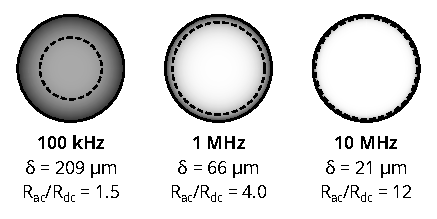
\includegraphics[width=\linewidth]{fig/lec01/skin_effect_wire.pdf}
				\caption{Current density in a round copper wire, 1\,mm diameter, 20\,$^\circ$C (exact solution; darker means higher $|J|$, dashed: one skin depth below the surface)}
			\end{figure}
		\end{column}
		\begin{column}{0.47\textwidth}
			Skin depth of copper:
			\begin{equation*}
				\delta=\sqrt{\frac{\rho}{\pi f \mu_0}}\approx\frac{66\,\mu\mathrm{m}}{\sqrt{f/\mathrm{MHz}}}\quad(20\,^\circ\mathrm{C})
			\end{equation*}
			\small
			\begin{itemize}
				\item 1\,oz PCB copper (35\,$\mu$m) equals $\delta$ at 3.6\,MHz.
				\item At 100\,$^\circ$C: $\rho$ +31\,\%, $\delta$ +15\,\%.
				\item In multilayer windings the proximity effect adds far more loss (Dowell, L7).
				\item Litz wire loses its advantage above a few MHz: the finest strands (50\,AWG, 25\,$\mu$m) equal $\delta$ at 7\,MHz.
			\end{itemize}
		\end{column}
	\end{columns}
	\blfootnote{Sources: Perreault, APEC 2024 plenary; Dowell, Proc. IEE, 1966.}
\end{frame}

%%%%%%%%%%%%%%%%%%%%%%%%%%%%%%%%%%%%%%%%%%%%%%%%%%%%%%%%%%%%%
%% Your turn: skin depth %%
%%%%%%%%%%%%%%%%%%%%%%%%%%%%%%%%%%%%%%%%%%%%%%%%%%%%%%%%%%%%%
% Two pages: task (page 1) and task with solution (page 2).
\begin{frame}<handout:1-2>
	\frametitle{Skin depth at 6.78\,MHz}
	\begin{block}{Task (3 minutes)}
		A single-layer copper foil winding carries a 6.78\,MHz current. The magnetic field is on one side of the foil only.
		\begin{enumerate}
			\item Skin depth of copper at 20\,$^\circ$C?
			\item Which copper thickness do you choose: 1\,oz (35\,$\mu$m) or 2\,oz (70\,$\mu$m)?
		\end{enumerate}
	\end{block}
	\onslide<2-|handout:2>{
		\begin{enumerate}
			\item $\delta=66\,\mu\mathrm{m}/\sqrt{6.78}\approx 25\,\mu$m.
			\item 1\,oz. For a single layer with the field on one side, the AC resistance is lowest at a thickness of $\frac{\pi}{2}\delta\approx 40\,\mu$m. 1\,oz is within 2\,\% of this optimum. 2\,oz gives about 7.5\,\% more AC resistance than 1\,oz: the extra copper carries almost no current. The derivation follows in L7 (Dowell).
		\end{enumerate}
	}
\end{frame}

%%%%%%%%%%%%%%%%%%%%%%%%%%%%%%%%%%%%%%%%%%%%%%%%%%%%%%%%%%%%%
%% Timing %%
%%%%%%%%%%%%%%%%%%%%%%%%%%%%%%%%%%%%%%%%%%%%%%%%%%%%%%%%%%%%%
\begin{frame}
	\frametitle{Timing at high frequency}
	\begin{columns}[T]
		\begin{column}{0.47\textwidth}
			\begin{figure}
				\centering
				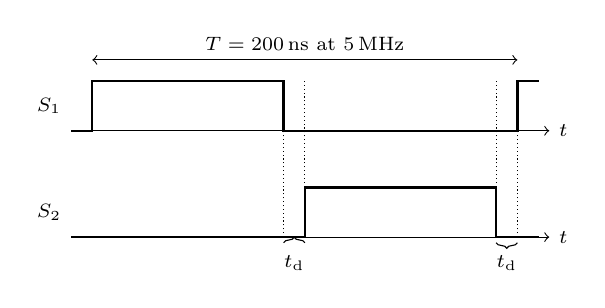
\begin{tikzpicture}[x=0.027cm, y=0.9cm]
					% time axes
					\draw[->] (0,0) -- (225,0) node[right, font=\scriptsize] {$t$};
					\draw[->] (0,1.5) -- (225,1.5) node[right, font=\scriptsize] {$t$};
					% gate signal S1 (high side): on from 10 ns to 100 ns and from 210 ns
					\draw[thick] (0,1.5) -- (10,1.5) -- (10,2.2) -- (100,2.2) -- (100,1.5) -- (210,1.5) -- (210,2.2) -- (220,2.2);
					% gate signal S2 (low side): on from 110 ns to 200 ns
					\draw[thick] (0,0) -- (110,0) -- (110,0.7) -- (200,0.7) -- (200,0) -- (220,0);
					\node[anchor=east, font=\scriptsize] at (0,1.85) {$S_1$};
					\node[anchor=east, font=\scriptsize] at (0,0.35) {$S_2$};
					% dead times
					\draw[densely dotted] (100,0) -- (100,2.2) (110,0) -- (110,2.2);
					\draw[densely dotted] (200,0) -- (200,2.2) (210,0) -- (210,2.2);
					\draw[decorate, decoration={brace, amplitude=2pt}] (100,-0.08) -- (110,-0.08) node[pos=0.5, below=1pt, font=\scriptsize] {$t_\mathrm{d}$};
					\draw[decorate, decoration={brace, mirror, amplitude=2pt}] (200,-0.08) -- (210,-0.08) node[pos=0.5, below=1pt, font=\scriptsize] {$t_\mathrm{d}$};
					% period
					\draw[<->] (10,2.5) -- node[above, font=\scriptsize] {$T=200$\,ns at 5\,MHz} (210,2.5);
				\end{tikzpicture}
				\caption{Gate signals of a half-bridge at 5\,MHz with $t_\mathrm{d}=10$\,ns (to scale)}
			\end{figure}
		\end{column}
		\begin{column}{0.5\textwidth}
			\small
			\begin{itemize}
				\item Two dead times of 10\,ns already take 10\,\% of the period at 5\,MHz.
				\item Drivers and digital isolators add delays of tens of ns. Their part-to-part spread must fit into the dead time.
				\item A duty-cycle resolution of 0.1\,\% at 5\,MHz needs a time step of 0.2\,ns, i.e.\ a 5\,GHz counter or a high-resolution PWM unit.
				\item Isolated drivers must tolerate the switch-node $\mathrm{d}v/\mathrm{d}t$: their common-mode transient immunity (CMTI) must exceed e.g.\ 100\,V/ns.
			\end{itemize}
			Sensing and control are often not the limit. If they are, avoid controls that need low latency (L13).
		\end{column}
	\end{columns}
	\blfootnote{Source: Perreault, APEC 2024 plenary.}
\end{frame}

%%%%%%%%%%%%%%%%%%%%%%%%%%%%%%%%%%%%%%%%%%%%%%%%%%%%%%%%%%%%%
%% Quiz: what limits miniaturisation %%
%%%%%%%%%%%%%%%%%%%%%%%%%%%%%%%%%%%%%%%%%%%%%%%%%%%%%%%%%%%%%
% Two pages: question (page 1) and answer (page 2).
\begin{frame}<handout:1-2>
	\frametitle{What limits miniaturisation?}
	A 1\,kW converter is redesigned from 100\,kHz to 10\,MHz. Which two items limit the size reduction most? Vote, then discuss with your neighbour (2 minutes).
	\begin{enumerate}[(a)]
		\item the control loop and the sensing
		\item the magnetic components
		\item the device losses ($C_\mathrm{oss}$ loss, dynamic $R_\mathrm{DS(on)}$)
		\item the EMI filter
	\end{enumerate}
	\onslide<2-|handout:2>{
		\begin{block}{Answer: (b) and (c)}
			Core loss limits $\hat{B}$ and the skin effect limits the useful copper, so magnetics shrink much less than $1/f_\mathrm{sw}$. $C_\mathrm{oss}$ losses remain with soft switching and can exceed the conduction loss. The EMI filter becomes smaller as $f_\mathrm{sw}$ rises, and sensing and control are often not the limiting factor.
		\end{block}
	}
	\blfootnote{Source: Perreault, APEC 2024 plenary.}
\end{frame}

%%%%%%%%%%%%%%%%%%%%%%%%%%%%%%%%%%%%%%%%%%%%%%%%%%%%%%%%%%%%%
%% Summary table %%
%%%%%%%%%%%%%%%%%%%%%%%%%%%%%%%%%%%%%%%%%%%%%%%%%%%%%%%%%%%%%
\begin{frame}
	\frametitle{Summary of scaling laws}
	\begin{table}
		\centering
		\small
		\begin{tabular}{|l|l|>{\raggedright\arraybackslash}p{5.9cm}|}
			\hline
			\textbf{Quantity}                     & \textbf{Scaling}                   & \textbf{Remark}                                                      \\
			\hline
			Required $L$ and $C$                  & $\propto 1/f_\mathrm{sw}$          & for a given ripple                                                   \\
			EMI filter $LC$                       & $\propto 1/f_\mathrm{sw}^2$        & for a given attenuation at $f_\mathrm{sw}$                           \\
			Control bandwidth                     & $\propto f_\mathrm{sw}$            & crossover at about $f_\mathrm{sw}/10$                                \\
			Hard-switching loss                   & $\propto f_\mathrm{sw}$            & $Q_\mathrm{oss}V_\mathrm{DC}$, overlap, gate charge, dead time       \\
			Core loss density at fixed $\hat{B}$  & $\propto f_\mathrm{sw}^{\alpha}$   & $\alpha\approx 1.4$--$2$ for ferrites, so $\hat{B}$ must fall         \\
			Power density of magnetics            & rises, then falls                  & optimum at 10--30\,MHz, set by the material                          \\
			Skin depth                            & $\propto 1/\sqrt{f_\mathrm{sw}}$   & $R_\mathrm{ac}$ rises, litz wire loses its advantage                 \\
			Parasitics, delays, dead time         & fixed in ns                        & their share of the period grows with $f_\mathrm{sw}$                 \\
			Conduction loss                       & independent                        & $I^2R_\mathrm{DS(on)}$                                               \\
			\hline
		\end{tabular}
		\caption{First-order scaling laws of this lecture ($\alpha$ after Perreault et al., 2009)}
	\end{table}
\end{frame}

%%%%%%%%%%%%%%%%%%%%%%%%%%%%%%%%%%%%%%%%%%%%%%%%%%%%%%%%%%%%%
%% Consequences and roadmap %%
%%%%%%%%%%%%%%%%%%%%%%%%%%%%%%%%%%%%%%%%%%%%%%%%%%%%%%%%%%%%%
\subsection{Consequences and course roadmap}

\begin{frame}
	\frametitle{Need for soft switching}
	\begin{columns}[T]
		\begin{column}{0.52\textwidth}
			Capacitive switching loss relative to the output power:
			\begin{equation*}
				\frac{P_\mathrm{Qoss}}{P_\mathrm{o}}=\frac{Q_\mathrm{oss}V_\mathrm{DC}f_\mathrm{sw}}{P_\mathrm{o}}
			\end{equation*}
			For the 650\,V GaN device at 400\,V and 1\,kW, this reaches 1\,\% at 625\,kHz.\\[0.2em]
			Three ways to raise $f_\mathrm{sw}$ anyway:
			\begin{enumerate}
				\item zero-voltage switching: an inductive current commutates the switch-node voltage before the switch turns on (L8--L10)
				\item lower voltage per switch: multilevel, stacked and switched-capacitor converters (L12)
				\item better devices: less $Q_\mathrm{oss}$ and $C_\mathrm{oss}$ hysteresis for the same $R_\mathrm{DS(on)}$ (L2)
			\end{enumerate}
		\end{column}
		\begin{column}{0.45\textwidth}
			\begin{block}{What soft switching does not remove}
				\begin{itemize}
					\item $C_\mathrm{oss}$ hysteresis loss
					\item gate-drive loss
					\item core and winding loss
					\item conduction loss of the circulating current
				\end{itemize}
			\end{block}
			Hence the commutation cell, gate drive, measurement and magnetics (L2--L7) come before the soft-switching and resonant topologies (L8--L10).
		\end{column}
	\end{columns}
\end{frame}

%%%%%%%%%%%%%%%%%%%%%%%%%%%%%%%%%%%%%%%%%%%%%%%%%%%%%%%%%%%%%
%% Course roadmap %%
%%%%%%%%%%%%%%%%%%%%%%%%%%%%%%%%%%%%%%%%%%%%%%%%%%%%%%%%%%%%%
\begin{frame}
	\frametitle{Course roadmap}
	\begin{columns}[T]
		\begin{column}{0.49\textwidth}
			\footnotesize
			\begin{tabular}{|l|l|>{\raggedright\arraybackslash}p{4.7cm}|}
				\hline
				L1 & 13.10. & Why high switching frequency?                                  \\
				L2 & 20.10. & HF switching cell: losses and devices     \\
				L3 & 27.10. & Parasitics and PCB layout              \\
				L4 & 03.11. & Gate drivers for fast-switching devices                        \\
				L5 & 10.11. & Measurement and characterisation                         \\
				L6 & 17.11. & HF magnetics I: materials, core loss       \\
				L7 & 24.11. & HF magnetics II: windings, planar      \\
				L8 & 01.12. & Soft switching without resonance                               \\
				\hline
			\end{tabular}
		\end{column}
		\begin{column}{0.49\textwidth}
			\footnotesize
			\begin{tabular}{|l|l|>{\raggedright\arraybackslash}p{4.7cm}|}
				\hline
				L9  & 08.12. & Resonant converters I: SRC, PRC, LLC, CLLC                    \\
				L10 & 15.12. & Resonant converters II: VHF, matching \\
				L11 & 22.12. & Case studies and teardown                                     \\
				L12 & 12.01. & Switched-capacitor and hybrid converters                      \\
				L13 & 19.01. & Modelling and control at HF                                   \\
				L14 & 26.01. & EMI, thermal design and integration                           \\
				L15 & 02.02. & Synthesis and exam preparation               \\
				\hline
			\end{tabular}
		\end{column}
	\end{columns}
	\vspace{0.4cm}
	Tutorials on Wednesdays, 08--10, from 14.10. Each tutorial has a Jupyter notebook. T1 starts with the frequency-scaling explorer and the set-up of Python, ngspice and KiCad.
\end{frame}

%%%%%%%%%%%%%%%%%%%%%%%%%%%%%%%%%%%%%%%%%%%%%%%%%%%%%%%%%%%%%
%% Key messages %%
%%%%%%%%%%%%%%%%%%%%%%%%%%%%%%%%%%%%%%%%%%%%%%%%%%%%%%%%%%%%%
\begin{frame}
	\frametitle{Key messages}
	\begin{enumerate}
		\item The energy per cycle falls with $1/f_\mathrm{sw}$, and so do the required $L$ and $C$. EMI filters and control bandwidth benefit even more.
		\item Components do not shrink in proportion: core loss limits $\hat{B}$, skin and proximity effect limit the useful copper, and small magnetics are inherently less efficient.
		\item Every hard switching event costs $Q_\mathrm{oss}V_\mathrm{DC}$ plus overlap, gate and dead-time energy. Somewhere between a few hundred kHz (high voltage) and a few MHz (low voltage), this energy must be recovered by soft switching.
		\item Parasitics and delays are fixed in nanoseconds and take a growing share of the period.
		\item $f_\mathrm{sw}$ is a design variable with an optimum, not a goal in itself.
	\end{enumerate}
\end{frame}

%%%%%%%%%%%%%%%%%%%%%%%%%%%%%%%%%%%%%%%%%%%%%%%%%%%%%%%%%%%%%
%% Exit ticket %%
%%%%%%%%%%%%%%%%%%%%%%%%%%%%%%%%%%%%%%%%%%%%%%%%%%%%%%%%%%%%%
% Two pages: questions (page 1) and answers (page 2).
\begin{frame}<handout:1-2>
	\frametitle{Exit ticket}
	\begin{varblock}[\textwidth]{Three questions, one minute each}
		\begin{enumerate}
			\item You raise $f_\mathrm{sw}$ from 200\,kHz to 2\,MHz. By which factor can the $LC$ product of a second-order EMI filter shrink for the same attenuation at $f_\mathrm{sw}$?
			\item Name two loss mechanisms that remain with zero-voltage switching.
			\item Skin depth of copper (20\,$^\circ$C) at 1\,MHz and at 100\,MHz?
		\end{enumerate}
	\end{varblock}
	\onslide<2-|handout:2>{
		\begin{enumerate}
			\item By 100: the corner frequency can rise by 10, and $LC\propto 1/f_\mathrm{c}^2$.
			\item Any two of: $C_\mathrm{oss}$ hysteresis, gate drive, conduction (including circulating current), core and winding loss.
			\item 66\,$\mu$m and 6.6\,$\mu$m.
		\end{enumerate}
	}
\end{frame}

%%%%%%%%%%%%%%%%%%%%%%%%%%%%%%%%%%%%%%%%%%%%%%%%%%%%%%%%%%%%%
%% Recommended reading %%
%%%%%%%%%%%%%%%%%%%%%%%%%%%%%%%%%%%%%%%%%%%%%%%%%%%%%%%%%%%%%
\begin{frame}
	\frametitle{Recommended reading}
	\small
	\begin{itemize}
		\item J.\,G. Kassakian, D.\,J. Perreault, G.\,C. Verghese, M.\,F. Schlecht, \textit{Principles of Power Electronics}, 2nd ed., Cambridge University Press, 2023.
		\item R.\,W. Erickson, D. Maksimovi\'c, \textit{Fundamentals of Power Electronics}, 3rd ed., Springer, 2020.
		\item M.\,K. Kazimierczuk, D. Czarkowski, \textit{Resonant Power Converters}, 2nd ed., Wiley, 2011.
		\item W.\,G. Hurley, W.\,H. W\"olfle, \textit{Transformers and Inductors for Power Electronics}, Wiley, 2013.
		\item A. Lidow, M. de Rooij, J. Strydom, D. Reusch, J. Glaser, \textit{GaN Transistors for Efficient Power Conversion}, 3rd ed., Wiley, 2019.
		\item F. Wang, Z. Zhang, E.\,A. Jones, \textit{Characterization of Wide Bandgap Power Semiconductor Devices}, IET, 2018.
		\item Z. Zhang, Y.-F. Liu, \textit{High Frequency MOSFET Gate Drivers}, IET, 2017.
		\item H.\,W. Ott, \textit{Electromagnetic Compatibility Engineering}, Wiley, 2009.
	\end{itemize}
	The papers used in each lecture are listed at its end.
\end{frame}

%%%%%%%%%%%%%%%%%%%%%%%%%%%%%%%%%%%%%%%%%%%%%%%%%%%%%%%%%%%%%
%% References of this lecture %%
%%%%%%%%%%%%%%%%%%%%%%%%%%%%%%%%%%%%%%%%%%%%%%%%%%%%%%%%%%%%%
\begin{frame}
	\frametitle{References}
	\scriptsize
	\begin{itemize}
		\item D.\,J. Perreault, ``Opportunities, progress and challenges in high-frequency power conversion,'' plenary talk, IEEE APEC 2024.
		\item D.\,J. Perreault et al., ``Opportunities and challenges in very high frequency power conversion,'' IEEE APEC 2009, pp.\ 1--14.
		\item J.\,W. Kolar et al., ``PWM converter power density barriers,'' IEEJ Trans.\ Ind.\ Appl., vol.\ 128, no.\ 4, pp.\ 468--480, 2008.
		\item D. Neumayr et al., ``The essence of the Little Box Challenge -- Part A: Key design challenges \& solutions,'' CPSS Trans.\ Power Electron.\ Appl., vol.\ 5, no.\ 2, pp.\ 158--179, 2020.
		\item C.\,R. Sullivan, B.\,A. Reese, A.\,L.\,F. Stein, P.\,A. Kyaw, ``On size and magnetics: Why small efficient power inductors are rare,'' 3D-PEIM 2016.
		\item A.\,J. Hanson et al., ``Measurements and performance factor comparisons of magnetic materials at high frequency,'' IEEE Trans.\ Power Electron., vol.\ 31, no.\ 11, pp.\ 7909--7925, 2016.
		\item G. Zulauf et al., ``COSS losses in 600 V GaN power semiconductors in soft-switched, high- and very-high-frequency power converters,'' IEEE Trans.\ Power Electron., vol.\ 33, no.\ 12, pp.\ 10748--10763, 2018.
		\item J.\,B. Fedison, M. Fornage, M.\,J. Harrison, D.\,R. Zimmanck, ``Coss related energy loss in power MOSFETs used in zero-voltage-switched applications,'' IEEE APEC 2014, pp.\ 150--156.
		\item P.\,L. Dowell, ``Effects of eddy currents in transformer windings,'' Proc.\ IEE, vol.\ 113, no.\ 8, pp.\ 1387--1394, 1966.
		\item Y. Zhang et al., ``Wide-bandgap semiconductors and power electronics as pathways to carbon neutrality,'' Nature Reviews Electrical Engineering, vol.\ 2, pp.\ 155--172, 2025.
	\end{itemize}
\end{frame}

\begin{frame}
	\frametitle{References (cont.)}
	\scriptsize
	Designs in the MHz table and on the power--frequency map:
	\begin{itemize}
		\item E.\,A. Burton et al., ``FIVR -- Fully integrated voltage regulators on 4th generation Intel Core SoCs,'' IEEE APEC 2014, pp.\ 432--439.
		\item Y. Elasser et al., ``Mini-LEGO: A 1.5-MHz 240-A 48-V-to-1-V CPU VRM with 8.4-mm height for vertical power delivery,'' IEEE APEC 2023, pp.\ 1959--1966.
		\item M.\,K. Ranjram, D.\,J. Perreault, ``A 380-12 V, 1-kW, 1-MHz converter using a miniaturized split-phase, fractional-turn planar transformer,'' IEEE Trans.\ Power Electron., vol.\ 37, no.\ 2, pp.\ 1666--1681, 2022.
		\item S. Lim, D.\,M. Otten, D.\,J. Perreault, ``New AC--DC power factor correction architecture suitable for high-frequency operation,'' IEEE Trans.\ Power Electron., vol.\ 31, no.\ 4, 2016.
		\item J. Santiago-Gonz\'alez et al., ``Single-phase universal-input PFC converter operating at high frequency,'' IEEE J.\ Emerg.\ Sel.\ Topics Ind.\ Electron., 2023.
		\item L. Gu et al., ``6.78-MHz wireless power transfer with self-resonant coils at 95\,\% DC--DC efficiency,'' IEEE Trans.\ Power Electron., vol.\ 36, no.\ 3, pp.\ 2456--2460, 2021.
		\item H. Zhang, ``Techniques for efficient wide-range radio-frequency power generation,'' PhD thesis, MIT, 2022.
		\item Y. Cao et al., ``Design and implementation of an 18 kW 500 kHz 98.8\,\% efficiency high-density battery charger with partial power processing,'' IEEE J.\ Emerg.\ Sel.\ Topics Power Electron., vol.\ 10, pp.\ 7963--7975, 2022.
		\item Further wireless and RF power designs on the map (Braun 2019; Al Bastami 2020; Regensburger 2022; Nikiforidis 2023) as cited in Perreault, APEC 2024.
	\end{itemize}
\end{frame}
